Som det fremgår af \ref{antal_regioner_vertikale_cut} for det vertikale
plan, koncenterer regionerne sig omkring miden af billederne.

Graf \ref{antal_regioner_horisontale_cut} viser data for det
horisontale, plan. Hvor $92$ ligger højest. Fra miden af billedet og op
af bliver der fundet færre og færre regioner i snittene. Det skyldes at
billeder med horisont normalt har få regioner over horisonten, og mange
under, horisonten.

Graf \ref{antal_regioner_vertikale_cut} vise data for det vertikale,
plan. Grafen peaker i midden og falder hænd mod kanterne.

Hvis man samler informatioerne for de to grafer, kan man se at
regionerne samler sig fra den horisontale miden og ned af i billedet med
peaker i miden af det vertikalle plan. Det mod skrider hypotese
\ref{hypo_alle_andre_snit} og \ref{hypo_midten} og vi kan derfor
forkaste dem.

\begin{figure}[h!]
	\begin{center}
		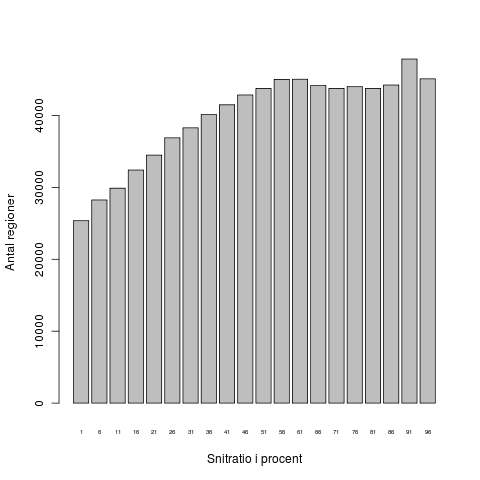
\includegraphics[width=0.9\textwidth]{afsnit/resultater/billeder/cut2cut3eatsperratio.png}
	\end{center}
	\caption{Antal regioner i hvert af de 20 horisontale snit, hvor venstre side af grafen repræsenterer øverst del af malerierne. $G$ står for det gyldne snit}
	\label{antal_regioner_horisontale_cut}
\end{figure}

\begin{figure}[h!]
	\begin{center}
		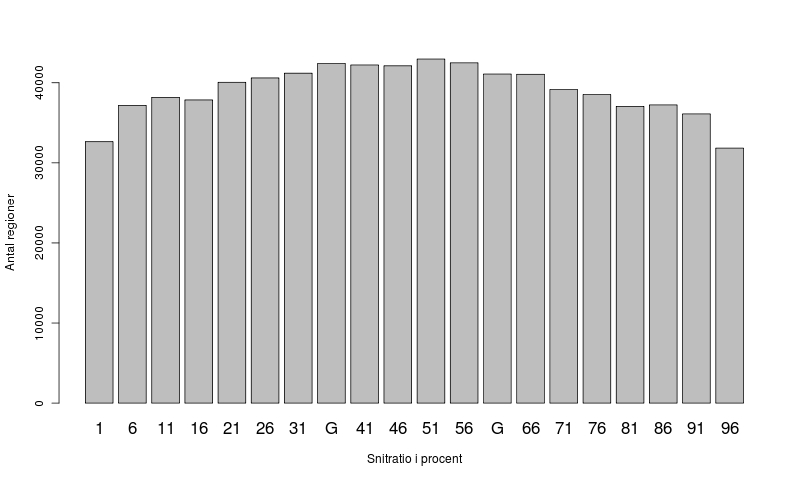
\includegraphics[width=0.9\textwidth]{afsnit/resultater/billeder/cut0cut1eatsperratio.png}
	\end{center}
	\caption{Antal regioner i hvert af de 20 vertikale snit. $G$ står for det gyldne snit}
	\label{antal_regioner_vertikale_cut}
\end{figure}

Graf \ref{G_vs_to_trejedele} vise forskellen på det gyldne snit og
$\frac{2}{3}$ i de fire snit. Som man kan se, er der ikke meget forskel
på det gyldne snit og $\frac{2}{3}$, og den største procentvise forskel
ligger på $2.34\%$. Da $2.34 \% < 15\%$, må vi sige at hypotese
\ref{hypo_15p} ikke, kan afviges.

I graf \ref{G_vs_to_trejedele}, kan man også se, at selv om snittene
ligger tæt på hinanden, så har det gyldne snit ca 2 procents sat
flere regioner. Vi kan derfor ikke afvise hypotese
\ref{hypo_to_tredjedele}

\begin{figure}[h!]
	\begin{center}
		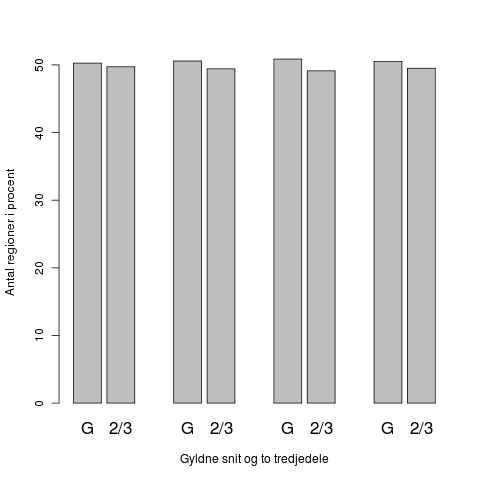
\includegraphics[width=0.6\textwidth]{afsnit/resultater/billeder/G_vs_to_tredjedele.png}
	\end{center}
	\caption{Procent vis antal regioner i de fire gyldne snit og deres tilhørene $\frac{2}{3}$ snit}
	\label{G_vs_to_trejedele}
\end{figure}

Grafen i figur \ref{naiv_year}, viser hvor mange regioner der
er fundet i gennemsnit per maleri i alle tidsperioder. Det ses at i
tidsperioden $(1301-1350)$ bliver der fundet ca 17 regioner per maleri,
som er klart flest. Tidsperioden (1200-1250) er den tidsperiode hvor der
bliver fundet færrest regioner, ca 7 i gennemsnit. Faktisk bliver der bliver fundet
mere en dobbelt så mange regioner i tidsperiode. Det betyder at
hypotese \ref{hypo_tid} kan forkastes.

\begin{figure}[!h]
	\begin{center}
		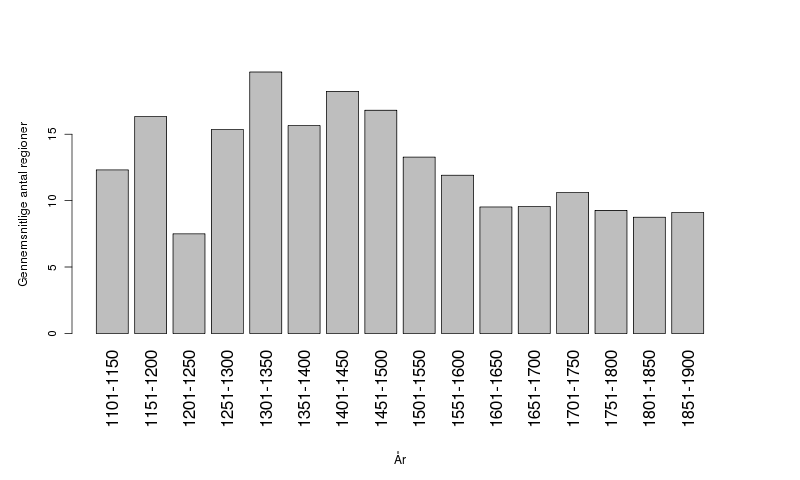
\includegraphics[angle=0,width=0.90\textwidth]{afsnit/resultater/billeder/yearcut.png}
	\end{center}
	\caption{Graf over gennemsnitligt antal regioner fundet for hver
       tidsperiode. Hver bjælke repræsenterer et land. Y-aksen er
       det gemmesnitlige antal fundene regioner i snittet.}
	\label{naiv_year}
\end{figure}

\begin{figure}[!h]
	\begin{center}
		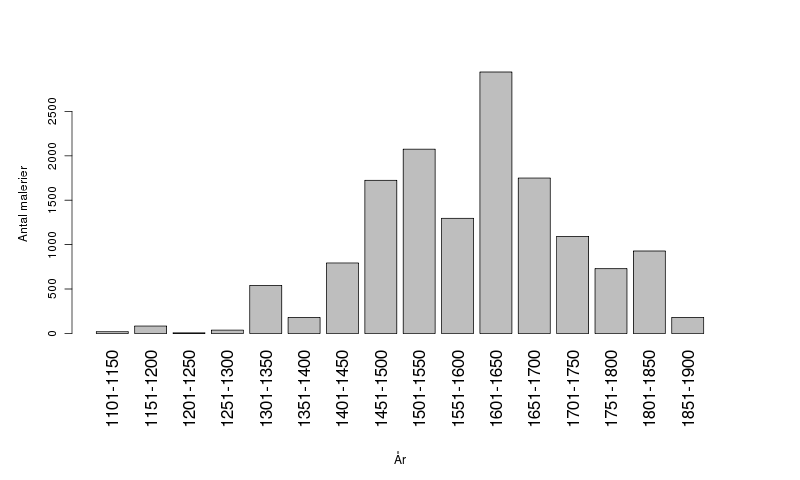
\includegraphics[angle=0,width=0.90\textwidth]{afsnit/resultater/billeder/yearNrImage.png}
	\end{center}
	\caption{}
	\label{naiv_yearNrImage}
\end{figure}

I graferne i figur \ref{naiv_nation}, vises samme repræsentation som
\ref{naiv_year}, blot er det her nationer i stedet for år. Nationerne
Greek, Holland og Catala har har klart flest regioner per billede, hvor
imod Norge og Skotland ligger i bunden. Forskellen på disse nation
ligger på ca 12 regioner,hvilket svarer til en forskel på ca $240\%$. Da
$240 \% > 10 \%$ holder hypotese \ref{hypo_nation} ikke.

\begin{figure}[!h]
	\begin{center}
		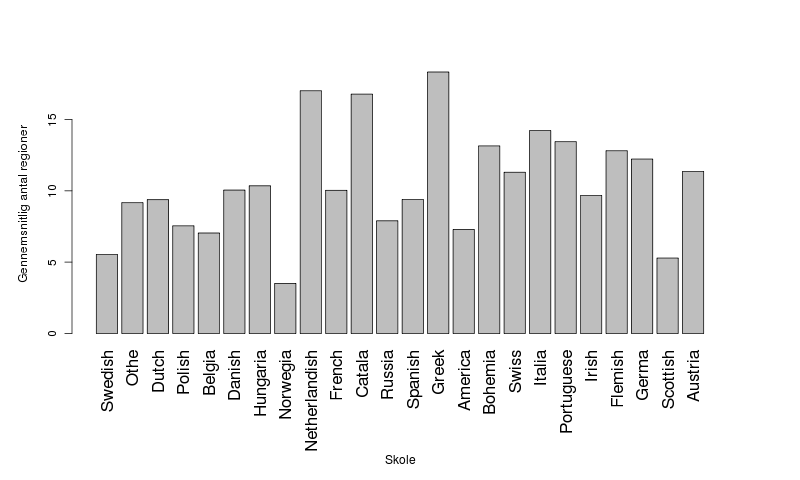
\includegraphics[angle=0,width=0.90\textwidth]{afsnit/resultater/billeder/nationcut.png}
	\end{center}
	\caption{Graf over gennemsnitligt antal fundne regioner fundet hver sin
       nationalitet. Hver bjælke repræsenterer et tidsinterval. Y-aksen
       er det gemmesnitlige antal fundne regioner i snittet.}
	\label{naiv_nation}
\end{figure}

\begin{figure}[!h]
	\begin{center}
		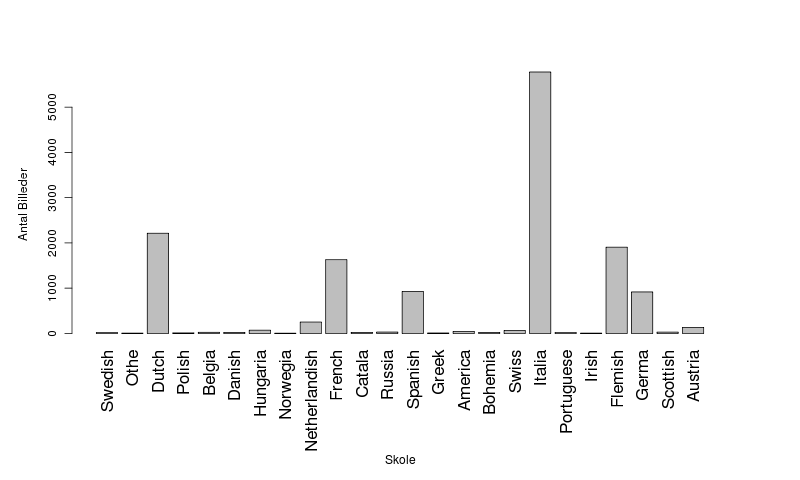
\includegraphics[angle=0,width=0.90\textwidth]{afsnit/resultater/billeder/nationNrImage.png}
	\end{center}
	\caption{}
	\label{naiv_nationNrImage}
\end{figure}

